\documentclass[11pt,oneside]{book}

\usepackage{hyperref}
\usepackage{graphicx}
\usepackage{listings}
\usepackage{xcolor} % Use xcolor for more color options
\usepackage{tikz}
\usepackage[margin=1in]{geometry}
\usepackage{titlesec}
\usepackage[most]{tcolorbox} % Load tcolorbox with 'most' library for more features
\usepackage{fancyhdr}
\usepackage{enumitem}
\usepackage{caption}
\usepackage{soul}
\usepackage{array}
\usepackage{amsmath}
\usepackage{amssymb} % Added for math symbols
\usepackage{booktabs}
\usepackage{tabularx} % For tables with adjusted width columns

% --- Adjust Headheight for fancyhdr ---
\setlength{\headheight}{14pt} % Increased from default to accommodate header content

% --- Color Definitions ---
\definecolor{codegreen}{rgb}{0,0.6,0}
\definecolor{codegray}{rgb}{0.5,0.5,0.5}
\definecolor{codepurple}{rgb}{0.58,0,0.82}
\definecolor{backcolour}{rgb}{0.95,0.95,0.92}
\definecolor{hlyellow}{HTML}{FFFACD} % yellow!40 approx
\definecolor{hlred}{HTML}{FFCCCB} % red!20 approx
\definecolor{hlblue}{HTML}{ADD8E6} % blue!20 approx

% --- Listing Styles ---
\lstdefinestyle{mystyle}{
    backgroundcolor=\color{backcolour},
    commentstyle=\color{codegreen},
    keywordstyle=\color{magenta},
    numberstyle=\tiny\color{codegray},
    stringstyle=\color{codepurple},
    basicstyle=\ttfamily\footnotesize,
    breakatwhitespace=false,
    breaklines=true,
    captionpos=b,
    keepspaces=true,
    numbers=left,
    numbersep=5pt,
    showspaces=false,
    showstringspaces=false,
    showtabs=false,
    tabsize=2,
    mathescape=true % Added to allow math mode in listings like in boolean.tex
}
\lstset{style=mystyle}

% --- Highlighting Command ---
\newcommand{\hlc}[2][hlyellow]{\sethlcolor{#1}\hl{#2}}

% --- TColorBox Setup ---
\tcbset{
    colback=blue!5!white,
    colframe=blue!75!black,
    fonttitle=\bfseries
}

% --- Title Formatting ---
\titleformat{\chapter}{\normalfont\huge\bfseries}{\thechapter}{20pt}{\huge}
\titlespacing*{\chapter}{0pt}{-30pt}{20pt} % Adjust spacing as needed

% --- Header/Footer ---
\pagestyle{fancy}
\fancyhf{} % Clear default headers/footers
\fancyhead[R]{\leftmark} % Chapter title on the right header
\fancyfoot[C]{\thepage} % Page number in the center footer
\renewcommand{\headrulewidth}{0.4pt} % Add a line under the header
\renewcommand{\footrulewidth}{0pt} % No line above the footer

% --- Hyperref Setup ---
\hypersetup{
    colorlinks=true,
    linkcolor=blue,
    filecolor=magenta,
    urlcolor=cyan,
    pdftitle={AP Computer Science Principles Summary},
    pdfpagemode=FullScreen,
}

% --- Document Title ---
% Removed helper commands, placing text directly
\title{AP Computer Science Principles \\ Summary}
\author{\href{https://rowi.dev/}{Robin Wiethüchter} (AI Assisted)}
\date{\today}

% --- Document Start ---
\begin{document}
% Replace \maketitle with a custom titlepage that includes the disclaimer
\begin{titlepage}
    \centering
    \vspace*{2cm}
    
    {\LARGE\bfseries AP Computer Science Principles \\ Summary\par}
    \vspace{1cm}
    {\large\href{https://rowi.dev/}{Robin Wiethüchter} (AI Assisted)\par}
    \vspace{1cm}
    {\large\today\par}
    
    \vspace{2cm}
    
    % Disclaimer box
    \fbox{\parbox{0.8\textwidth}{
    \centering
    \large\textbf{DISCLAIMER: WORK IN PROGRESS}\\[0.5em]
    \normalsize This document is currently under development. Sections may be incomplete, contain errors, or be subject to significant changes.
    }}
\end{titlepage}

\frontmatter % Use frontmatter for ToC, etc.
\tableofcontents

\mainmatter % Start main content

% =============================================
% Chapter 1: Creative Development
% =============================================
\chapter{Big Idea 1: Creative Development}
\label{chap:creative_development}

The process of developing computational artifacts (like programs, digital images, audio, video, presentations, or web pages) is iterative and often collaborative. This Big Idea explores how computing innovations are created and their potential impacts.

\section{Collaboration}
\label{sec:collaboration}
Developing complex computational artifacts often requires collaboration, where individuals bring diverse perspectives and skills. Effective collaboration includes:
\begin{itemize}
    \item Communication: Clearly explaining ideas, progress, and problems.
    \item Shared Goals: Working towards a common objective.
    \item Contribution: Each member actively participates.
    \item Conflict Resolution: Addressing disagreements constructively.
    \item Using Tools: Employing version control (like Git) or shared document platforms to manage contributions.
\end{itemize}

\section{Program Function and Purpose}
\label{sec:program_function_purpose}
Every program or computational artifact is designed with a specific purpose and function.
\begin{itemize}
    \item \textbf{Purpose}: The problem the program aims to solve or the creative expression it intends to convey (e.g., calculating grades, simulating planetary motion, creating interactive art).
    \item \textbf{Function}: What the program actually does; the specific tasks it performs (e.g., takes user input, performs calculations, displays output, responds to events).
\end{itemize}
Understanding the intended purpose helps guide the development process and evaluate the final product.

\section{Program Design and Development}
\label{sec:program_design_development}
This is an iterative process involving cycles of designing, implementing, testing, and refining. Key phases include:
\begin{enumerate}[label=\arabic*.]
    \item \textbf{Investigation/Understanding the Problem}: Defining the requirements, purpose, and target audience.
    \item \textbf{Design}: Planning the program's structure, algorithms, user interface, and data representation. This might involve pseudocode, flowcharts, or diagrams.
    \item \textbf{Implementation (Coding)}: Writing the program code in a chosen programming language.
    \item \textbf{Testing}: Identifying and fixing errors (debugging). This involves running the program with various inputs and scenarios.
    \item \textbf{Refinement}: Improving the program based on testing, feedback, or new requirements. This could involve adding features, optimizing performance, or enhancing usability.
    \item \textbf{Documentation}: Explaining how the program works, how to use it, and the design choices made. This can include comments in the code and external documents.
\end{enumerate}
This process is rarely linear; developers often loop back to earlier phases.

\section{Identifying and Correcting Errors (Debugging)}
\label{sec:debugging}
Errors (bugs) are inevitable in programming. Debugging strategies include:
\begin{itemize}
    \item \textbf{Testing}: Systematically checking program behavior with different inputs.
    \item \textbf{Reading Error Messages}: Understanding compiler/interpreter messages.
    \item \textbf{Print Statements/Logging}: Inserting temporary output commands to track program flow and variable values.
    \item \textbf{Using a Debugger Tool}: Step-by-step execution, inspecting variables, setting breakpoints.
    \item \textbf{Simplifying the Problem}: Isolating the error by commenting out code sections or testing smaller parts.
\end{itemize}
Different types of errors exist:
\begin{itemize}
    \item \textbf{Syntax Errors}: Violations of the programming language's grammar rules (caught by the compiler/interpreter).
    \item \textbf{Runtime Errors}: Errors occurring during program execution (e.g., division by zero, accessing invalid memory).
    \item \textbf{Logic Errors}: The program runs but produces incorrect results because the algorithm or its implementation is flawed. These are often the hardest to find.
\end{itemize}

\textbf{Overflow Error}: Computers use a fixed number of bits (e.g., 8 bits) to represent numbers. This limits the largest value they can store (for 8 bits, often 255). An overflow error happens when a calculation's result is too large for the available bits. When this occurs, the result often "wraps around." For example, adding 1 to the maximum value might result in 0, or even a negative number if signed numbers are being used. This unexpected wrap-around leads to incorrect results.

\textbf{Round-off Error}: Similarly, computers use a finite number of bits to represent real numbers (like decimals or fractions), which can have infinite precision. This means computers often store an \textit{approximation} rather than the exact value. This small difference is called a round-off error. While often tiny, these errors can accumulate during calculations, potentially leading to noticeable inaccuracies in the final result (e.g., 0.1 + 0.2 might be stored as something like 0.30000000000000004 instead of exactly 0.3).

% =============================================
% Chapter 2: Data
% =============================================
\chapter{Big Idea 2: Data}
\label{chap:data}
% Placeholder for Big Idea 2 content
Computers store, process, and transmit information digitally using binary data. This Big Idea focuses on how data is represented, manipulated, and used.

\section{Bits and Bytes}
\label{sec:bits_bytes}
The fundamental unit of digital information is the \textbf{bit} (binary digit), which can represent one of two states: 0 or 1. Bits are grouped together to represent more complex data.
\begin{itemize}
    \item \textbf{Byte}: A group of 8 bits. A common unit for measuring data size.
    \item \textbf{Number of States}: With $n$ bits, you can represent $2^n$ distinct states or values. For example, 8 bits (1 byte) can represent $2^8 = 256$ different values (often 0-255).
\end{itemize}

\section{Number Systems}
\label{sec:number_systems}
Computers use binary internally, but humans often use other systems for convenience.
\begin{itemize}
    \item \textbf{Binary (Base-2)}: Uses only digits 0 and 1. Each position represents a power of 2 (e.g., $1101_2 = 1*2^3 + 1*2^2 + 0*2^1 + 1*2^0 = 8 + 4 + 0 + 1 = 13_{10}$).
    \item \textbf{Decimal (Base-10)}: The system we use daily, with digits 0-9. Each position represents a power of 10.
\end{itemize}

\textbf{Overflow Error}: Computers use a fixed number of bits (e.g., 8 bits) to represent numbers. This limits the largest value they can store (for 8 bits, often 255). An overflow error happens when a calculation's result is too large for the available bits. When this occurs, the result often "wraps around." For example, adding 1 to the maximum value might result in 0, or even a negative number if signed numbers are being used. This unexpected wrap-around leads to incorrect results.

\textbf{Round-off Error}: Similarly, computers use a finite number of bits to represent real numbers (like decimals or fractions), which can have infinite precision. This means computers often store an \textit{approximation} rather than the exact value. This small difference is called a round-off error. While often tiny, these errors can accumulate during calculations, potentially leading to noticeable inaccuracies in the final result (e.g., 0.1 + 0.2 might be stored as something like 0.30000000000000004 instead of exactly 0.3).

% Figure: Binary to Decimal Conversion (simplified to match image)
\begin{figure}[h!]
    \centering
    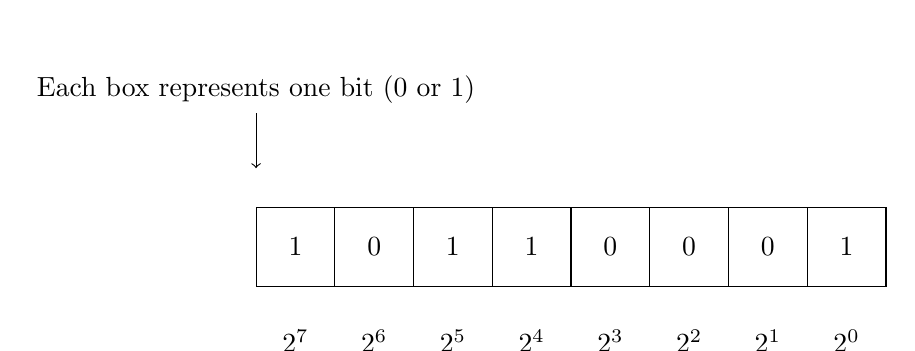
\begin{tikzpicture}
        % Title text
        \node at (0,2) {Each box represents one bit (0 or 1)};
        \draw[->] (0,1.7) -- (0,1);
        
        % Boxes with binary digits
        \foreach \i/\bit/\power in {0/1/7,1/0/6,2/1/5,3/1/4,4/0/3,5/0/2,6/0/1,7/1/0} {
            \draw (\i,-0.5) rectangle ++(1,1);
            \node at (\i+0.5,0) {\bit};
            \node at (\i+0.5,-1.2) {$2^{\power}$};
        }
    \end{tikzpicture}
    
    \vspace{1em}
    $1 \cdot 2^7 + 0 \cdot 2^6 + 1 \cdot 2^5 + 1 \cdot 2^4 + 0 \cdot 2^3 + 0 \cdot 2^2 + 0 \cdot 2^1 + 1 \cdot 2^0$\\
    $= 128 + 0 + 32 + 16 + 0 + 0 + 0 + 1$\\
    $= 177_{10}$
    
    \caption{Converting binary to decimal: Each bit's value is multiplied by its position value (powers of 2)}
    \label{fig:binary-byte}
\end{figure}

% Figure: Binary Addition (simplified to match image)
\begin{figure}[h!]
    \centering
    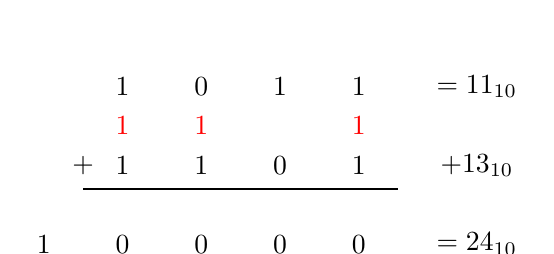
\begin{tikzpicture}
        % First number
        \node at (0,1) {1};
        \node at (1,1) {0};
        \node at (2,1) {1};
        \node at (3,1) {1};
        \node at (4.5,1) {$ = 11_{10}$};
        
        % Plus and second number
        \node at (-0.5,0) {$+$};
        \node[text=red] at (0,0.5) {1};
        \node at (0,0) {1};
        \node[text=red] at (1,0.5) {1};
        \node at (1,0) {1};
        \node at (2,0) {0};
        \node[text=red] at (3,0.5) {1};
        \node at (3,0) {1};
        \node at (4.5,0) {$ + 13_{10}$};
        
        % Line
        \draw (-0.5,-0.3) -- (3.5,-0.3);
        
        % Result
        \node at (-1,-1) {1};
        \node at (0,-1) {0};
        \node at (1,-1) {0};
        \node at (2,-1) {0};
        \node at (3,-1) {0};
        \node at (4.5,-1) {$ = 24_{10}$};
    \end{tikzpicture}
    \caption{Binary addition example (1011 + 1101 = 11000) showing carry bits in red}
    \label{fig:binary-addition}
\end{figure}

\section{Sampling and Representing Analog Data}
\label{sec:sampling}
To represent continuous, real-world phenomena (like sound waves or visual scenes) digitally, we need to convert them into discrete values. This involves:
\begin{itemize}
    \item \textbf{Sampling}: Measuring the phenomenon's value at regular intervals in either time (for sound) or space (for images). The \textbf{sampling rate} (or resolution) determines how frequently these measurements are taken. More samples generally lead to a more accurate representation but require more data.
\end{itemize}
This process inherently involves approximation, as the continuous reality is represented by discrete digital data. The number of bits used to store each sample (bit depth) determines the level of detail or number of distinct values that can be represented.

\subsection*{Representing Images}
Images are represented by sampling visual information across a 2D space. The image is divided into a grid of \textbf{pixels} (picture elements), each representing a sample point. For each pixel, color information is captured, often using RGB (Red, Green, Blue) values, each stored with a certain number of bits (bit depth) to represent different color intensities. Image file formats (JPEG, PNG, GIF) use different encoding and compression techniques.

\subsection*{Representing Sound}
Sound is represented by sampling an analog sound wave's amplitude (height) at regular time intervals (the sampling rate). Each sample's amplitude is then stored using a specific number of bits (bit depth). Higher sampling rates and bit depths capture the original sound more accurately, resulting in higher fidelity but larger file sizes.

\section{Data Compression}
\label{sec:data_compression}
Compression reduces the number of bits needed to store or transmit data.
\begin{itemize}
    \item \textbf{Lossless Compression}: Allows perfect reconstruction of the original data (e.g., ZIP, PNG). Algorithms look for redundancies (like repeated patterns) and encode them more efficiently.
    \item \textbf{Lossy Compression}: Discards some information deemed less important to achieve higher compression ratios (e.g., JPEG, MP3). This is acceptable for images and audio where humans may not notice the slight loss of quality. The original data cannot be perfectly recovered.
\end{itemize}
The choice depends on the data type and requirements (e.g., text needs lossless, video often uses lossy).

\section{Extracting Information from Data}
\label{sec:extracting_info}
Large datasets can reveal patterns, trends, and insights not obvious from individual data points. Techniques include:
\begin{itemize}
    \item \textbf{Filtering}: Selecting a subset of data based on criteria (e.g., show only sales from the last month).
    \item \textbf{Sorting}: Arranging data in a specific order (e.g., alphabetically, numerically).
    \item \textbf{Aggregation}: Summarizing data (e.g., calculating averages, sums, counts).
    \item \textbf{Visualization}: Creating charts and graphs (bar charts, scatter plots, heat maps) to make patterns easier to understand.
    \item \textbf{Data Mining / Machine Learning}: Using algorithms to discover complex patterns, make predictions, or classify data automatically.
\end{itemize}
Computers are essential for processing large datasets efficiently. These extraction techniques are often implemented using programming algorithms that iterate through data structures like lists (see Section \ref{sec:lists}) to filter, aggregate, or transform information based on specific criteria.

\begin{lstlisting}[language={}, label={lst:data_filtering_example}, caption={AP Pseudocode: Filtering Data in a List}]
// Example: Find all scores above 90 in a list
highScores <- [] // Create an empty list to store results
allScores <- [75, 92, 88, 95, 60, 100]

FOR EACH score IN allScores
{
    IF (score > 90)
    {
        APPEND(highScores, score) // Add score to the highScores list
    }
}

DISPLAY("High scores found:")
DISPLAY(highScores) // Output: [92, 95, 100]
\end{lstlisting}

\section{Digital Data Security and Privacy}
\label{sec:data_security_privacy}
Collecting and storing digital data raises significant concerns:
\begin{itemize}
    \item \textbf{Security}: Protecting data from unauthorized access, modification, or destruction (e.g., using passwords, encryption, firewalls).
    \item \textbf{Privacy}: Controlling how personal information is collected, used, and shared. This includes issues like data breaches, surveillance, and PII (Personally Identifiable Information).
    \item \textbf{Anonymization}: Removing PII from datasets to protect privacy while still allowing analysis. However, re-identification can sometimes be possible by combining anonymized data with other sources.
    \item \textbf{Metadata Concerns}: Even metadata (e.g., file creation times, locations in photos) can reveal sensitive information.
\end{itemize}

% =============================================
% Chapter 3: Algorithms and Programming
% =============================================
\chapter{Big Idea 3: Algorithms and Programming}
\label{chap:algorithms_programming}
% Placeholder for Big Idea 3 content
Programming enables us to implement algorithms that solve problems. This involves using programming languages to express instructions a computer can execute.

\section{Variables and Assignments}
\label{sec:variables_assignment}
Variables are named storage locations for data values that can change during program execution. You can think of a variable as a box with a label on it. We can look at what value is in the box or put a new value in the box.

\begin{itemize}
    \item \textbf{Declaration/Assignment}: In AP Pseudocode, variables are often declared implicitly when they are first assigned a value using the assignment operator (<-). In other languages, you might need to declare the type first.
    \begin{lstlisting}[language={}, label={lst:assignment_detail}, caption={AP Pseudocode: Assignment Examples}]
    x <- 5          // Assigns the value 5 to variable x
    y <- 10
    z <- x + y      // Assigns the value of x + y (15) to z
    message <- "Hello" // Assigns a string value
    isValid <- true   // Assigns a boolean value

    // Updating a variable's value
    x <- x + 1      // Reads the current value of x (5), adds 1, assigns the result (6) back to x
    \end{lstlisting}
    \item \textbf{Naming}: Meaningful variable names (e.g., \texttt{totalScore} instead of just \texttt{s}) significantly improve code readability and understanding.
\end{itemize}

\subsection*{Common Data Types in Programming}
Variables hold different kinds of data, known as data types. Common types include:
\begin{itemize}
    \item \textbf{Numbers}: Used for mathematical values. Can be integers (whole numbers, like `5`, `-10`) or real numbers (with decimals, like `3.14`). Internally represented using binary (see Section \ref{sec:number_systems}). Be aware of potential \textbf{overflow} and \textbf{round-off errors} (Section \ref{sec:number_systems}).
    \item \textbf{Text (Strings)}: Sequences of characters (letters, numbers, symbols) enclosed in quotes, like `"Hello"` or `"CSP2024"`. Characters are represented internally using standards like ASCII or Unicode.
    \item \textbf{Booleans}: Represent logical values, either `true` or `false`. Essential for making decisions in programs (see Section \ref{sec:control_structures}).
    \item \textbf{Lists (Arrays)}: Ordered collections of items, which can be of any data type (including other lists). Covered in detail in Section \ref{sec:lists}.
\end{itemize}
The type of data determines the operations that can be performed on it (e.g., you can do arithmetic on numbers, but not directly on strings).

\section{Mathematical and Logical Expressions}
\label{sec:expressions}
Programs use expressions, combining values, variables, and operators, to compute new values. Categories include:
\begin{itemize}
    \item Numbers, Strings, Variables
    \item \hlc[hlred]{Logical Operators}
    \item \hlc[hlyellow]{Relational Operators}
    \item \hlc[hlblue]{Parentheses}
\end{itemize}

\subsection*{Mathematical Expressions}
Use arithmetic operators to perform calculations.
\begin{itemize}
    \item Operators: \texttt{+}, \texttt{-}, \texttt{*}, \texttt{/}, \texttt{MOD} (modulus/remainder).
    \item Order of Operations: Follows standard mathematical precedence (PEMDAS/BODMAS). Parentheses \hlc[hlblue]{( )} can be used to force a specific evaluation order.
\end{itemize}
\begin{lstlisting}[language={}, label={lst:math_expr_detail}, caption={AP Pseudocode: Math Expressions}]
    totalCost <- price * quantity
    remainder <- 17 MOD 5 // remainder will be 2
    average <- (a + b + c) / 3 // Parentheses ensure addition happens before division
\end{lstlisting}

\subsection*{Relational Operators}
\hlc[hlyellow]{Relational operators} compare two values and evaluate to a Boolean result (\texttt{true} or \texttt{false}).

\begin{tabularx}{\textwidth}{>{\ttfamily}l >{\ttfamily}c X}
\toprule
\textbf{Code Symbol} & \textbf{AP Symbol} & \textbf{Meaning} \\
\midrule
\hlc[hlyellow]{==} (often) & \hlc[hlyellow]{=} & Equal to \\
\hlc[hlyellow]{!=} & \hlc[hlyellow]{$\neq$} & Not equal to \\
\hlc[hlyellow]{>} & \hlc[hlyellow]{>} & Greater than \\
\hlc[hlyellow]{<} & \hlc[hlyellow]{<} & Less than \\
\hlc[hlyellow]{>=} & \hlc[hlyellow]{$\geq$} & Greater than or equal to \\
\hlc[hlyellow]{<=} & \hlc[hlyellow]{$\leq$} & Less than or equal to \\
\bottomrule
\end{tabularx}

\subsection*{Logical Operators}
\hlc[hlred]{Logical operators} combine two or more Boolean expressions.

\begin{tabularx}{\textwidth}{>{\ttfamily}l >{\ttfamily}c X}
\toprule
\textbf{Code Symbol} & \textbf{AP Symbol} & \textbf{Meaning} \\
\midrule
\hlc[hlred]{\&\&} (often) & \hlc[hlred]{AND} & Logical AND (true only if \textit{both} operands are true) \\
\hlc[hlred]{||} (often) & \hlc[hlred]{OR} & Logical OR (true if \textit{at least one} operand is true) \\
\hlc[hlred]{!} (often) & \hlc[hlred]{NOT} & Logical NOT (evaluates to true if the operand is false, and vice versa) \\
\bottomrule
\end{tabularx}

\subsection*{Boolean Expression Examples}
\begin{itemize}
    \item \textit{Example 1:}
    \begin{lstlisting}[language={}, basicstyle=\ttfamily\small]
    (x > 10) AND (y < 20)
    \end{lstlisting}
    Evaluates to \texttt{true} if \texttt{x} is greater than 10 \textit{and} \texttt{y} is less than 20. (e.g., true for \texttt{x = 11, y = 19}; false for \texttt{x = 11, y = 21})
    \item \textit{Example 2:}
    \begin{lstlisting}[language={}, basicstyle=\ttfamily\small]
    NOT (a = b)
    \end{lstlisting}
    Evaluates to \texttt{true} if \texttt{a} is \textit{not} equal to \texttt{b}. (e.g., true for \texttt{a = 5, b = 2}; false for \texttt{a = 11, b = 11})
    \item \textit{Example 3 (Combined):}
    \begin{lstlisting}[language={}, basicstyle=\ttfamily\small]
    (score >= 70 AND score < 100) OR (isBonusEligible = true)
    \end{lstlisting}
    Evaluates to \texttt{true} if the score is between 70 (inclusive) and 100 (exclusive), \textit{or} if the student is eligible for a bonus.
\end{itemize}

\subsection*{Operator Comparison (JavaScript vs AP Pseudocode)}
Different programming languages may use different symbols for the same operation.

\begin{tabularx}{\textwidth}{l >{\ttfamily}l >{\ttfamily}l}
\toprule
\textbf{Operation} & \textbf{Common Code (e.g., JS)} & \textbf{AP Pseudocode} \\
\midrule
Assignment & x = 5 & x <- 5 \\
Equal to & \hlc[hlyellow]{a == b} & \hlc[hlyellow]{a = b} \\
Not Equal to & \hlc[hlyellow]{a != b} & \hlc[hlyellow]{a $\neq$ b} \\
Logical OR & \hlc[hlred]{a || b} & \hlc[hlred]{a OR b} \\
Logical AND & \hlc[hlred]{a \&\& b} & \hlc[hlred]{a AND b} \\
Logical NOT & \hlc[hlred]{!a} & \hlc[hlred]{NOT a} \\
\bottomrule
\end{tabularx}

\section{Control Structures}
\label{sec:control_structures}
Control structures determine the order in which instructions are executed.
\begin{itemize}
    \item \textbf{Sequence}: Instructions are executed one after another in the order they appear.
    \item \textbf{Selection (Conditionals)}: Executes different blocks of code based on a Boolean condition. Uses \texttt{IF}, \texttt{ELSE IF}, \texttt{ELSE}. (See details below)
    \item \textbf{Iteration (Loops)}: Repeats a block of code multiple times. (See details below)
\end{itemize}

\subsection*{Selection / Conditionals (Detailed)}

\subsubsection*{Basic IF Statement}
Executes a block of code only if a condition is true.
\begin{lstlisting}[language={}, label={lst:basic_if}, caption={AP Pseudocode: Basic IF}]
    IF (condition)
    {
        // Statements executed if condition is true
        statements
    }
    // Code here executes regardless
\end{lstlisting}
Example:
\begin{lstlisting}[language={}]
    score <- 100
    IF (score = 100) // Note: AP uses = for comparison
    {
        DISPLAY("Perfect score!")
    }
\end{lstlisting}

\subsubsection*{IF-ELSE Statement}
Executes one block of code if the condition is true, and a different block if the condition is false.
\begin{lstlisting}[language={}, label={lst:if_else}, caption={AP Pseudocode: IF-ELSE}]
    IF (condition)
    {
        // Statements executed if condition is true
        statements_if_true
    }
    ELSE
    {
        // Statements executed if condition is false
        statements_if_false
    }
\end{lstlisting}
Example:
\begin{lstlisting}[language={}]
    temperature <- 15
    IF (temperature > 20)
    {
        DISPLAY("It's warm.")
    }
    ELSE
    {
        DISPLAY("It's cool.") // This will be displayed
    }
\end{lstlisting}

\subsubsection*{IF - ELSE IF - ELSE Statement}
Checks multiple conditions in order. The first condition that evaluates to true has its corresponding block executed. If none are true, the optional \texttt{ELSE} block is executed.
\begin{lstlisting}[language={}, label={lst:if_elseif_else}, caption={AP Pseudocode: IF - ELSE IF - ELSE}]
    IF (condition1)
    {
        // Statements executed if condition1 is true
        statements1
    }
    ELSE IF (condition2)
    {
        // Statements executed if condition1 is false AND condition2 is true
        statements2
    }
    ELSE // Optional
    {
        // Statements executed if all preceding conditions are false
        statements_else
    }
\end{lstlisting}
Example (Grading):
\begin{lstlisting}[language={}, label={lst:grading_example}]
    score <- 85
    grade <- ""
    IF (score >= 90)
    {
        grade <- "A"
    }
    ELSE IF (score >= 80)
    {
        grade <- "B" // This block executes, grade becomes "B"
    }
    ELSE IF (score >= 70)
    {
        grade <- "C"
    }
    ELSE
    {
        grade <- "D"
    }
    DISPLAY(grade)
\end{lstlisting}
\textbf{Important:} Only one block (the first one whose condition is met) in an IF-ELSE IF-...-ELSE structure will execute.

\subsubsection*{Multiple Independent IF Statements}
Unlike ELSE IF, separate IF statements are evaluated independently.
\begin{lstlisting}[language={}, label={lst:multiple_if}, caption={AP Pseudocode: Multiple Independent IFs}]
    score <- 100
    count <- 0
    IF (score >= 80) // Condition is true
    {
        count <- count + 1 // count becomes 1
    }
    // This IF is checked regardless of the previous one
    IF (score >= 90) // Condition is true
    {
        count <- count + 1 // count becomes 2
    }
    count <- count + 1 // count becomes 3 (unconditional)
    // This IF is also checked independently
    IF (score >= 100) // Condition is true
    {
        count <- count + 1 // count becomes 4
    }
    DISPLAY(count) // Displays 4
\end{lstlisting}
Here, multiple IF blocks can execute if their respective conditions are true.

\subsubsection*{Nested Conditionals}
An IF statement can be placed inside another IF or ELSE block.
\begin{lstlisting}[language={}, label={lst:nested_if}, caption={AP Pseudocode: Nested IFs}]
    homeworkComplete <- true
    score <- 95
    grade <- ""

    IF (homeworkComplete = true) // Outer condition
    {
        // This block executes only if homeworkComplete is true
        DISPLAY("Checking score because homework is complete...")
        IF (score >= 90) // Inner condition
        {
            grade <- "A" // This executes
        }
        ELSE
        {
            grade <- "B"
        }
    }
    ELSE
    {
        grade <- "Incomplete"
    }
    DISPLAY(grade) // Displays "A"
\end{lstlisting}
Indentation helps visualize the structure of nested blocks.

\subsection*{Iteration / Loops (Detailed)}
Loops repeat blocks of code.
\begin{itemize}
    \item \textbf{\texttt{REPEAT n TIMES}}: Executes the block a fixed number of times.\\[1ex]
    \begin{lstlisting}[language={}, label={lst:repeat_n_detail}, caption={AP Pseudocode: REPEAT n TIMES}]
    count <- 0
    REPEAT 5 TIMES
    {
        count <- count + 1
        DISPLAY(count) // Displays 1, 2, 3, 4, 5
    }
    \end{lstlisting}
    \item \textbf{\texttt{REPEAT UNTIL (condition)}}: Executes the block \textit{first}, then checks the condition. Repeats as long as the condition is \texttt{false}. The block always executes at least once.\\[1ex]
    \begin{lstlisting}[language={}, label={lst:repeat_until_detail}, caption={AP Pseudocode: REPEAT UNTIL}]
    input <- ""
    REPEAT UNTIL (input = "quit")
    {
        DISPLAY("Enter command (or 'quit'):")
        input <- INPUT()
        // Process input...
        DISPLAY("You entered: " + input)
    }
    DISPLAY("Exiting loop.")
    \end{lstlisting}
    \item \textbf{\texttt{FOR EACH item IN list}} (Covered more in Lists): Iterates through each element in a list sequentially.\\[1ex]
    \begin{lstlisting}[language={}, label={lst:for_each_detail}, caption={AP Pseudocode: FOR EACH}]
    names <- ["Alice", "Bob", "Charlie"]
    FOR EACH name IN names
    {
        DISPLAY("Hello, " + name)
    }
    \end{lstlisting}
\end{itemize}
These three structures (Sequence, Selection, Iteration) are the fundamental building blocks for constructing any algorithm.

\section{Algorithms}
\label{sec:algorithms}
An algorithm is a finite sequence of well-defined, computer-implementable instructions to solve a class of problems or perform a computation.
% \begin{itemize}
%     \item \textbf{Clarity}: Steps must be unambiguous.
%     \item \textbf{Effectiveness}: Steps must be executable.
%     \item \textbf{Finiteness}: Must eventually terminate.
%     \item \textbf{Correctness}: Must produce the correct output for all valid inputs.
% \end{itemize}
Algorithms can be expressed in natural language, flowcharts, or pseudocode before being implemented in a programming language.

\section{Procedures (Functions/Methods)}
\label{sec:procedures}
Procedures (often called functions or methods) are named blocks of code that perform a specific task. They help organize code, reduce redundancy, and improve reusability.
\begin{itemize}
    \item \textbf{Definition}: Specifies the procedure name, parameters (inputs), and the code it executes.
    \item \textbf{Parameters}: Variables listed in the definition that receive values when the procedure is called.
    \item \textbf{Arguments}: The actual values passed to the parameters when the procedure is called.
    \item \textbf{Return Values}: Procedures can optionally return a value back to the calling code using the \texttt{RETURN} statement.
    \item \textbf{Modularity}: Breaking down a complex problem into smaller, manageable procedures.
    \item \textbf{Abstraction}: Hiding the complex details of implementation behind a simple interface (the procedure call).
\end{itemize}
\begin{lstlisting}[language={}, label={lst:procedure}, caption={AP Pseudocode: Procedure Definition and Call}]
// Procedure Definition
PROCEDURE calculateArea(length, width)
{
    area <- length * width
    RETURN(area)
}

// Procedure Call
roomLength <- 10
roomWidth <- 8
roomArea <- calculateArea(roomLength, roomWidth)
DISPLAY("The area is: ")
DISPLAY(roomArea)
\end{lstlisting}
When `calculateArea` is called, the value of `roomLength` (10) is passed as the argument for the `length` parameter, and `roomWidth` (8) is passed as the argument for the `width` parameter. Inside the procedure, these values are used to calculate `area`. The `RETURN(area)` statement sends the calculated value (80) back to where the procedure was called. This returned value is then assigned to the `roomArea` variable.

\section{Lists (Arrays)}
\label{sec:lists}
Lists (or arrays in some languages) are ordered collections of items (elements). AP Pseudocode uses 1-based indexing.
\begin{itemize}
    \item \textbf{Creating Lists}: \texttt{myList <- [item1, item2, item3]}
    \item \textbf{Accessing Elements}: By index. \texttt{firstItem <- myList[1]}, \texttt{thirdItem <- myList[3]}
    \item \textbf{Modifying Elements}: \texttt{myList[2] <- newItem}
    \item \textbf{Length}: Finding the number of elements. \texttt{len <- LENGTH(myList)}
    \item \textbf{Common Operations}: Adding items (\texttt{APPEND}), removing items (\texttt{REMOVE}), inserting items (\texttt{INSERT}).
    \item \textbf{Iteration with Lists}: Using \texttt{FOR EACH}.
    \begin{lstlisting}[language={}, label={lst:list_iteration}, caption={AP Pseudocode: List Iteration}]
    scores <- [85, 92, 78, 95]
    sum <- 0
    FOR EACH score IN scores
    {
        sum <- sum + score
    }
    average <- sum / LENGTH(scores)
    DISPLAY(average)
    \end{lstlisting}
\end{itemize}

\section{Algorithm Analysis}
\label{sec:algorithm_analysis}
Comparing algorithms that solve the same problem.
\begin{itemize}
    \item \textbf{Correctness}: Does the algorithm always produce the correct result?
    \item \textbf{Efficiency}: How many resources (time, memory) does the algorithm use, especially as the input size grows? Measured often using Big O notation (though not explicitly required by CSP, understanding relative efficiency is).
    \item \textbf{Readability/Simplicity}: Is the algorithm easy to understand and implement?
\end{itemize}
Different algorithms can have vastly different efficiencies. For example, linear search vs. binary search (requires sorted list).
\begin{itemize}
    \item \textbf{Linear Search}: Checks each element sequentially. Reasonable for small or unsorted lists. In the worst case, it takes a number of steps proportional to the size of the list (approximately n steps if the list has n items).
    \item \textbf{Binary Search}: Efficiently finds items in \textit{sorted} lists by repeatedly dividing the search interval in half. It compares the target value to the middle element; if they don't match, it eliminates half the list where the item cannot be and repeats the process on the remaining half. Much faster than linear search for large lists, taking significantly fewer steps (proportional to log n steps) for a list of size n.
\end{itemize}
\textbf{Heuristics}: Sometimes, finding an exact, optimal solution is too slow (computationally intractable). A heuristic is an approach that finds an approximate solution that is "good enough" for practical purposes, often much faster.

\textbf{Undecidable Problem}: A problem for which no algorithm can be constructed that always leads to a correct yes-or-no answer for every possible input (e.g., the Halting Problem - determining whether an arbitrary program will eventually stop running or continue forever).

\section{Simulations}
\label{sec:simulations}
Simulations use computer models to mimic real-world phenomena or systems. They allow us to:
\begin{itemize}
    \item Test hypotheses
    \item Explore complex systems where real-world experiments are impossible, dangerous, or expensive
    \item Make predictions
\end{itemize}
Simulations involve designing models with specific rules, variables, and interactions, often incorporating randomness (using random number generators) to reflect real-world variability.

% =============================================
% Chapter 4: Computer Systems and Networks
% =============================================
\chapter{Big Idea 4: Computer Systems and Networks}
\label{chap:systems_networks}
% Placeholder for Big Idea 4 content
Computing requires hardware and software working together. Networks, especially the Internet, connect computers globally, enabling communication and information sharing.

\section{Computer Components}
\label{sec:computer_components}
While CSP focuses less on deep hardware details, a basic understanding is helpful.
\begin{itemize}
    \item \textbf{Hardware}: The physical parts (CPU, memory/RAM, storage devices like HDDs/SSDs, input devices like keyboards/mice, output devices like monitors/printers).
    \item \textbf{Software}: Instructions that tell the hardware what to do (Operating Systems like Windows/macOS/Linux, Applications like browsers/word processors).
    \item \textbf{CPU (Central Processing Unit)}: Executes program instructions.
    \item \textbf{Memory (RAM)}: Temporary storage for data and programs currently in use. Volatile (data lost when power is off).
    \item \textbf{Storage}: Permanent storage for data and programs (Hard Drives, Solid State Drives). Non-volatile.
\end{itemize}
Hardware and software interact through layers of abstraction.

\section{The Internet}
\label{sec:internet}
The Internet is a global network of interconnected computer networks. It's a system for communication and information exchange.
\begin{itemize}
    \item \textbf{Decentralized}: No single point of control or failure.
    \item \textbf{Interoperability}: Uses standardized, open protocols (rules for communication) allowing different types of devices and networks to connect.
    \item \textbf{World Wide Web (WWW)}: A system of linked hypertext documents accessed via the Internet (using protocols like HTTP/HTTPS). The Web is *part* of the Internet, not the same thing. \textbf{Crucially, the Internet is the underlying network infrastructure (hardware and protocols), while the WWW is an information system built on top of the Internet.}
\end{itemize}

\section{How the Internet Works}
\label{sec:how_internet_works}
Data travels across the Internet using standardized procedures (protocols). Key concepts:
\begin{itemize}
    \item \textbf{Protocols}: Standardized sets of rules governing communication. Open protocols (like those used on the Internet) allow different types of devices and networks to connect and interoperate smoothly.
    \item \textbf{IP Addresses}: Every device connected to the Internet needs a unique numerical label, its IP address (Internet Protocol address), to be identified and receive data.
    \item \textbf{Domain Name System (DNS)}: Since remembering numerical IP addresses is difficult, the DNS acts like the Internet's phonebook. It translates human-readable domain names (e.g., \texttt{www.google.com}) into the corresponding IP addresses needed for routing.
    \item \textbf{Packets}: Data sent over the Internet is broken down into small units called packets. Each packet contains a portion of the data plus metadata (like source/destination IP addresses) needed for routing and reassembly.
    \item \textbf{Routing}: Devices called routers examine packet destination addresses and forward them across networks towards their destination. The Internet is designed to be dynamic; packets from the same message might take different routes depending on network conditions and efficiency.
    \item \textbf{Packet Reliability}: Protocols like TCP (Transmission Control Protocol) ensure reliable data transfer by managing packet sequencing, checking for errors, and requesting retransmission of lost packets. Other protocols like UDP prioritize speed over guaranteed delivery for applications like streaming. (You don't need to know the deep specifics of TCP/UDP, just that mechanisms exist for reliability vs. speed trade-offs).
    \item \textbf{World Wide Web (WWW) and HTTP/HTTPS}: The WWW is a system of linked information (web pages, files, etc.) accessed \textit{via} the Internet. It uses the HTTP (Hypertext Transfer Protocol) or HTTPS (secure version) to request and display web content. The WWW is one of many services that run on the Internet, but it is not the Internet itself.
    \item \textbf{Scalability}: The Internet's design using open protocols, packet switching, and decentralized routing allows it to expand to handle ever-increasing numbers of users and devices effectively.
\end{itemize}

\section{Fault Tolerance}
\label{sec:fault_tolerance}
Systems that can continue operating even if some components fail are fault-tolerant. The Internet achieves fault tolerance through:
\begin{itemize}
    \item \textbf{Redundancy}: Multiple paths exist between networks. If one path or router fails, traffic can often be automatically redirected through alternative routes.
    \item \textbf{Packet Switching}: Because data is broken into independent packets, if some packets are lost or take a faulty route, they can often be re-sent or rerouted without losing the entire message (especially when using reliable protocols like TCP).
\end{itemize}
This design makes the Internet robust against many common failures, ensuring communication can continue.

% Figure: Network Redundancy (from unit2.tex)
\begin{figure}[h!]
    \centering
    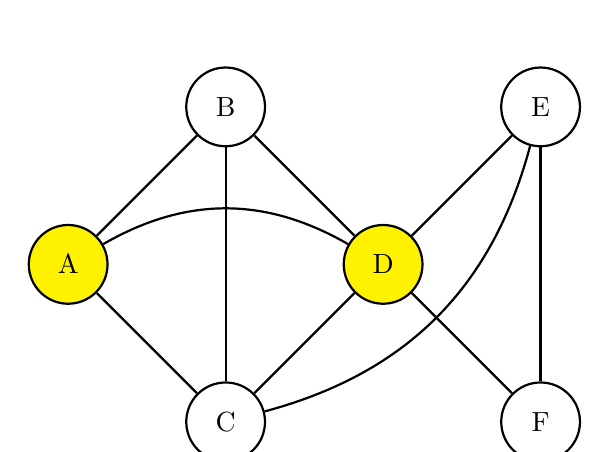
\begin{tikzpicture}[every node/.style={circle, draw, minimum size=1cm, inner sep=0pt}, thick]
        % Define nodes with highlighted A and D
        \node[fill=yellow] (A) at (0,0) {A};
        \node (B) at (2,2) {B};
        \node (C) at (2,-2) {C};
        \node[fill=yellow] (D) at (4,0) {D};
        \node (E) at (6,2) {E};
        \node (F) at (6,-2) {F};

        % Define undirected connections
        \draw (A) -- (B);
        \draw (A) -- (C);
        \draw (B) -- (C);
        \draw (B) -- (D);
        \draw (C) -- (D);
        \draw (D) -- (E);
        \draw (D) -- (F);
        \draw (E) -- (F);

        % Additional paths for redundancy - simplified slightly
        \draw (A) to [bend left=30] (D); % Direct redundant path A->D visualization
        \draw (C) to [bend right=30] (E); % Other redundancy example C->E

    \end{tikzpicture}
    \captionsetup{list=no} % Prevent figure from appearing in List of Figures if used
    \caption{
        Network diagram illustrating redundancy and fault tolerance. Multiple paths exist between nodes (e.g., A to D directly, via B, or via C). If one path (e.g., A-B-D) fails, data can be rerouted through another (e.g., A-C-D or the direct A-D path), allowing the network to continue functioning.
    }
    \label{fig:network-redundancy}
\end{figure}

\section{Parallel and Distributed Computing}
\label{sec:parallel_distributed}
These approaches use multiple computers or processors to solve large problems faster.
\begin{itemize}
    \item \textbf{Parallel Computing}: Uses multiple processors working simultaneously on parts of the same task, often within a single computer system.
    \item \textbf{Distributed Computing}: Spreads tasks across multiple, independent computers connected by a network (like the Internet). Examples include large-scale scientific simulations (e.g., protein folding) or big data processing.
    \item \textbf{Speedup}: The performance gain achieved by using parallel/distributed systems compared to a single processor. Ideally, $N$ processors could provide $N$ times speedup, but communication overhead and task dependencies often limit this.
\end{itemize}

\section{Cybersecurity}
\label{sec:cybersecurity}
Protecting computer systems, networks, and data from unauthorized access, attacks, damage, or theft.
\begin{itemize}
    \item \textbf{CIA Triad}: Core security goals:
        \begin{itemize}
            \item \textbf{Confidentiality}: Preventing unauthorized disclosure of information (achieved via encryption, access controls).
            \item \textbf{Integrity}: Ensuring data is accurate and hasn't been tampered with (achieved via hashing, digital signatures).
            \item \textbf{Availability}: Ensuring systems and data are accessible when needed (achieved via redundancy, backups, denial-of-service protection).
        \end{itemize}
    \item \textbf{Common Threats}:
        \begin{itemize}
            \item \textbf{Malware}: Malicious software (viruses, worms, ransomware, spyware).
            \item \textbf{Phishing}: Tricking users into revealing sensitive information (passwords, credit card numbers) often via deceptive emails, messages, or websites designed to look legitimate. \hlc[hlred]{(Frequently Tested!)}
            \item \textbf{Denial-of-Service (DoS/DDoS) Attacks}: Overwhelming a system with traffic to make it unavailable to legitimate users.
            \item \textbf{Rogue Access Point}: An unauthorized wireless access point installed on a network, potentially allowing attackers to intercept traffic or gain unauthorized access.
            \item \textbf{Keylogger}: Malware or hardware that records keystrokes entered on a keyboard, often used to steal passwords or other sensitive information.
            \item \textbf{Social Engineering}: Manipulating people to gain access or information.
        \end{itemize}
    \item \textbf{Countermeasures}:
        \begin{itemize}
            \item \textbf{Authentication}: Verifying identity (passwords, biometrics).
                \begin{itemize}
                    \item \textbf{Multifactor Authentication (MFA)}: Enhances security by requiring two or more distinct pieces of evidence (factors) to verify identity (e.g., something you know like a password + something you have like a code from your phone).
                \end{itemize}
            \item \textbf{Encryption}: Scrambling data (plaintext) into an unreadable format (ciphertext) using an algorithm and a key, so it's unintelligible without the key. Used for secure communication (HTTPS) and data storage.
                \begin{itemize}
                    \item \textbf{Symmetric Key Encryption}: Uses the \textbf{same secret key} for both encryption and decryption. Faster, but requires a secure way to share the secret key beforehand between the sender and receiver.
                    \item \textbf{Public Key (Asymmetric) Encryption}: Uses \textbf{two keys}: a \textit{public key} (shared freely) for encryption and a corresponding \textit{private key} (kept secret by the owner) for decryption. Anyone can encrypt a message using the recipient's public key, but only the recipient with the matching private key can decrypt it. This solves the key sharing problem of symmetric encryption but is computationally slower.
                        \begin{itemize}
                            \item \textbf{Public Key}: Can be shared with anyone without compromising security. Used to encrypt messages intended for the owner of the corresponding private key.
                            \item \textbf{Private Key}: Must be kept secret by the owner. Used to decrypt messages encrypted with the corresponding public key.
                        \end{itemize}
                \end{itemize}
            \begin{figure}[h!]
                \centering
                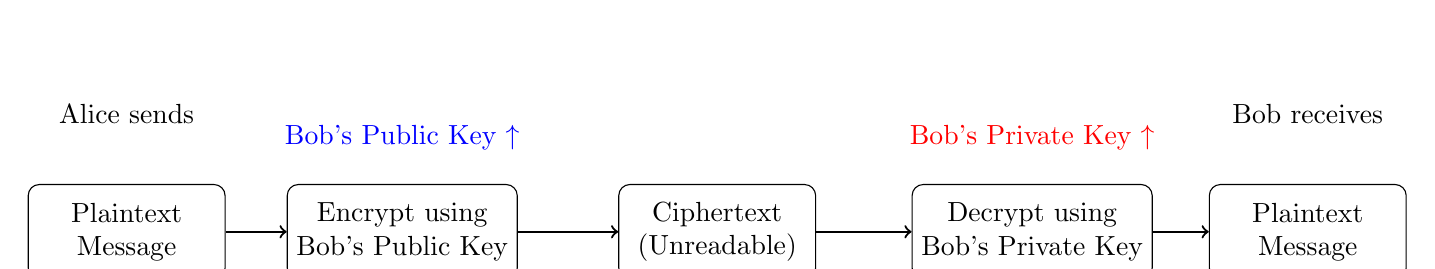
\begin{tikzpicture}[every node/.style={draw, rounded corners, align=center, minimum height=1.2cm, minimum width=2.5cm}]
                    % Define node coordinates explicitly
                    \node (Message)   at (0,0)   {Plaintext\\Message};
                    \node (Encrypt)   at (3.5,0)  {Encrypt using\\Bob's Public Key};
                    \node (Ciphertext)at (7.5,0)  {Ciphertext\\(Unreadable)};
                    \node (Decrypt)   at (11.5,0) {Decrypt using\\Bob's Private Key};
                    \node (Received)  at (15,0)  {Plaintext\\Message};
                    
                    % Alice and Bob labels 
                    \node (Alice) [draw=none, above of=Message, yshift=0.5cm] {Alice sends}; 
                    \node (Bob)   [draw=none, above of=Received, yshift=0.5cm] {Bob receives};

                    % Arrows
                    \draw[->, thick] (Message) -- (Encrypt);
                    \draw[->, thick] (Encrypt) -- (Ciphertext);
                    \draw[->, thick] (Ciphertext) -- (Decrypt);
                    \draw[->, thick] (Decrypt) -- (Received);
                    
                    % Key indication - positioned explicitly above Encrypt/Decrypt
                    \node (PubKey) [draw=none, text=blue, above of=Encrypt, yshift=0.2cm] {Bob's Public Key $\uparrow$}; 
                    \node (PrivKey) [draw=none, text=red, above of=Decrypt, yshift=0.2cm] {Bob's Private Key $\uparrow$};
                \end{tikzpicture}
                \caption{Public Key Encryption Example: Alice encrypts a message using Bob's public key. Only Bob, with his corresponding private key, can decrypt it.}
                \label{fig:public-key-encryption}
            \end{figure}
            \item \textbf{Firewalls}: Network security systems that monitor and control incoming/outgoing traffic based on rules.
            \item \textbf{Software Updates}: Patching vulnerabilities discovered in software.
            \item \textbf{User Education}: Awareness about phishing and safe practices.
        \end{itemize}
\end{itemize}
Cybersecurity is an ongoing challenge due to evolving threats and system complexity.

% =============================================
% Chapter 5: Impact of Computing
% =============================================
\chapter{Big Idea 5: Impact of Computing}
\label{chap:impact_computing}
% Placeholder for Big Idea 5 content
Computing technologies have profoundly changed society, bringing numerous benefits but also raising significant ethical and societal challenges.

\section{Beneficial Effects}
\label{sec:beneficial_effects}
Computing innovations have driven progress in many areas:
\begin{itemize}
    \item \textbf{Communication}: Facilitating instant global communication (email, social media, video conferencing).
    \item \textbf{Access to Information}: Providing vast resources for learning and research (World Wide Web, online libraries, search engines).
    \item \textbf{Collaboration}: Enabling collaboration on projects regardless of geographic location.
    \item \textbf{Creativity and Expression}: Offering new tools for art, music, writing, and design.
    \item \textbf{Automation}: Performing repetitive or dangerous tasks, increasing efficiency in various industries.
    \item \textbf{Economic Growth}: Creating new industries, jobs, and markets.
    \item \textbf{Scientific Advancement}: Enabling complex simulations, data analysis, and discovery in fields like medicine, climate science, and physics.
    \item \textbf{Crowdsourcing / Citizen Science}: Leveraging the skills, knowledge, or computing power of large numbers of people, often via the internet, to solve complex problems, gather data, or contribute to research (e.g., protein folding projects, identifying galaxies, transcribing historical documents).
    \item \textbf{Accessibility}: Providing assistive technologies for people with disabilities.
\end{itemize}

\section{Harmful Effects and Challenges}
\label{sec:harmful_effects}
Alongside benefits, computing raises concerns:
\begin{itemize}
    \item \textbf{Bias in Algorithms}: Algorithms, often trained on historical data, can reflect and amplify existing societal biases (e.g., in facial recognition, loan applications, hiring tools).
    \item \textbf{Privacy Concerns}: Widespread collection and analysis of personal data raise issues of surveillance, data breaches, and misuse of information.
    \item \textbf{Security Risks}: Increased reliance on digital systems makes individuals and infrastructure vulnerable to cyberattacks (as discussed in Big Idea 4).
    \item \textbf{Digital Divide}: Unequal access to computing devices, the internet, and digital literacy skills creates disparities in opportunities (economic, educational, social).
    \item \textbf{Workforce Impact}: Automation can displace workers in certain sectors, requiring workforce adaptation and retraining.
    \item \textbf{Information Reliability}: The ease of spreading information online makes it challenging to distinguish credible sources from misinformation and disinformation.
    \item \textbf{Intellectual Property}: Digital content (music, movies, software) is easily copied, leading to challenges in protecting copyright and preventing piracy.
    \item \textbf{Social Impacts}: Effects on social interaction, mental health (e.g., social media addiction), and the nature of community.
\end{itemize}

\section{Bias in Computing}
\label{sec:bias_computing}
Bias can be introduced into computing systems at various stages:
\begin{itemize}
    \item \textbf{Data Bias}: If the data used to train an algorithm is not representative of the population it will be used on, the algorithm may perform poorly or unfairly for certain groups.
    \item \textbf{Algorithm Bias}: The design choices made by programmers can inadvertently introduce bias.
    \item \textbf{Human Bias}: The people designing, implementing, and using technology can bring their own conscious or unconscious biases.
\end{itemize}
It's crucial to be aware of potential biases and strive to create and use technology equitably.

\section{Legal and Ethical Concerns}
\label{sec:legal_ethical}
Computing raises complex legal and ethical questions:
\begin{itemize}
    \item \textbf{Copyright and Intellectual Property}: How to balance creators' rights with public access to information and innovation. 
        \begin{itemize}
            \item \textbf{Copyright}: The legal right granted to the creator of original works (literature, music, software, etc.), usually for a limited time. It gives the creator exclusive rights to copy, distribute, and adapt the work. 
            \item \textbf{Open Source Software (OSS)}: Software for which the original source code (the human-readable instructions written by programmers) is made freely available and may be redistributed and modified. Users can see how the software works, fix bugs, or adapt it. This contrasts with proprietary software, where the source code is kept secret. Examples include the Linux operating system and the Firefox web browser. OSS licenses still have rules, but they prioritize sharing and modification.
            \item \textbf{Creative Commons (CC)}: A set of public copyright licenses that enable the free distribution of an otherwise copyrighted work. A creator uses a CC license to give others permission to share, use, and build upon their work, under certain conditions specified by the license (e.g., requiring attribution, prohibiting commercial use). This provides a more flexible alternative to the traditional "all rights reserved" copyright, facilitating sharing and collaboration, especially for digital content like images, music, and text.
            \item \textbf{Fair Use}: A legal doctrine that permits limited use of copyrighted material without permission from the rights holders for purposes such as criticism, comment, news reporting, teaching, scholarship, or research.
        \end{itemize}
    \item \textbf{Data Privacy Laws}: Regulations like GDPR (Europe) or CCPA (California) attempt to give individuals more control over their personal data.
    \item \textbf{Responsibility}: Who is responsible when an autonomous system (like a self-driving car) causes harm?
    \item \textbf{Ethical Use}: Considering the potential consequences of technology and using it responsibly.
\end{itemize}

\section{Safe Computing}
\label{sec:safe_computing}
Refers to practices for protecting oneself and one's data online.
\begin{itemize}
    \item \textbf{Strong Passwords \& Authentication}: Using unique, complex passwords and enabling multi-factor authentication where possible.
    \item \textbf{Recognizing Phishing}: Being wary of suspicious emails, links, or requests for personal information.
    \item \textbf{Secure Connections}: Using HTTPS websites (look for the padlock) and being cautious on public Wi-Fi.
    \item \textbf{Software Updates}: Keeping operating systems and applications updated to patch security vulnerabilities.
    \item \textbf{Data Backups}: Regularly backing up important files.
    \item \textbf{Privacy Settings}: Reviewing and adjusting privacy settings on social media and other online accounts.
    \item \textbf{Sharing Appropriately}: Being mindful of what personal information is shared online.
\end{itemize}

\end{document} 